\chapter{Design and Implementation - Retrieval}
\label{chapter:Design and Implementation - Retrieval}

\section{Random reads in HBase}

Unlike some Cloud-based databases which are optimized for random reads like PNUTS, HBase is write-optimized by using on-disk structure that can be maintained using sequential IO. Its records are never overwritten, instead, updates are written sequentially to new files in disk. That means that multiple updates of the same record will be spread over many files, so when reading it, multiple IO operations will be needed to merge the separate updates. On the other hand, as we already explained, all writing is sequential, so HBase excels at writing and consequently, in scans, which are sequential reads. This is a simple trade-off between optimizing for reads and optimizing for writes.

\subsection{Random reads in our heavy-write cluster}

In this section we test random reads for our HBase fully write-optimized cluster. In HBase, there is no big room for improving random reads, but still some improvements can be done to achieve a better random read performance than the default one.
\par
Before starting, we must describe how our reads are going to be, whether they will request an entire row, that will be the darkest room for enhancing it, or they will ask for a little part, better scenario as HBase stores familyColumns in separated files and only a few will be required in order to return the result. 
\par
The use case we performance is fetching 1, 10, 25, 50 or more random video details at once. The row keys of these random elements are known beforehand, so we only have to look for them and retrieve its details. In these reads, not all data is requested, but instead just the main data, which is within the first ColumnFamily (CF1).                  

\subsection{Studying random read performance}

Now that we have characterized reads, lets study a bit how we can enhance them. 
\par
First of all, the number of requested rows is really low if we compare with the total number of rows our data has, almost 45 millions counting duplicated ones. So we discard the idea of creating a \textit{Scan} object (previously described in HBase background chapter) instead of \textit{Gets} objects, since it will be helpful if we were requesting a high number of rows or if the keys would cover a small key range, but the row keys we are looking for do not represent it and above all, they are not sequential ones, so they are not even in the same region. Therefore, using \textit{Scan} would not help. 
\par
About whether to use Gets or Scan methods, Lars George, an authorized HBase voice, quantifies it specifying when it worths using one or the other. Its studies demonstrate that translating many \textit{Gets} into a \textit{Scan+Filter} is beneficial if the \textit{Scan} would return at least 1\%-2\% of the total rows to the client \footnote{ L. George Scan or Get study \newline \url{http://permalink.gmane.org/gmane.comp.java.hadoop.hbase.user/33133}}. In our particular case, in which we seek for a maximum of 50 rows, it only represents 0.00064\% of the total rows without the duplicates, so using \textit{Gets} will be likely more efficient.
\par
Another keypoint to keep in mind is that since the desired row keys are totally random, some times our lookups can be accesing most of the regions and others just hitting the same region. But this last thought is something we can not avoid, it depends upon the nature of the chosen row keys.
\par
One good idea could be using \textit{HBaseFilters} to limit the search. Filters allow to do fine-grained searches such as combing values bigger than X, rows with a certain timestamp, rows with a specified column, etc. But since all our rows have all columnFamiles completely filled and we merely want all the fields of a certain columnFamiliy there is no possibility to use filters to avoid some row seeks. Given the nature of our searches, we only need to look into a few HFiles, the ones containing the desired columnFamily. To narrow the scope of the search and thus speed up the process, we can use \textit{Get.addFamily()} method to just process the valid columnFamily files and no others. Its equivalent \textit{HBaseFilter} would be \textit{FamilyFilter} which filters on the columnFamily, but it is better to use the prior method.
\par

An additional improvement we can make is batching \textit{Gets} objects, instead of sending one by one. Using it is as simple as running the \textit{multi-get} method HBase supplies. We just need to write all the \textit{Get} instances within a list and then call \textit{Htable.get(List \textless{Get}\textgreater gets)}. Firstly, it sorts the requests by region server and subsequently goes serially to the region server to process the multi-get. It is done in a parallelized way across r egion servers. 
This method could be optimized by changing it to a multi-threading behavior. Instead of going one by one region server, it could sort the requests by region server as before, and then could spin up as many threads as targeted region servers, but it does not worth for our little multi-get operation.
%\cite{http://comments.gmane.org/gmane.comp.java.hadoop.hbase.user/34417}.
\par
Using HBase table as the source for a MapReduce job is discarded due to the little number of requested keys per examination. But of course it is another type of reading that HBase supports, which is incredibly useful in many situations. 


\subsection{Proceding with random read}

Once we have studied what our searches are going to require and how we must act, we can proceed. Our first try is simple, we create a list of \textit{Gets} objects (List \textless{Get}\textgreater gets), each one with a random key row obtained from a prior insertion, and we add them the columnFamily we want to check by calling to \textit{Get.addFamily()} method for each one. Then we execute it, \textit{Htable.get(List \textless{Get}\textgreater gets)}, and we measure the time it takes to carry out.


\begin{figure}[htb]
\centering
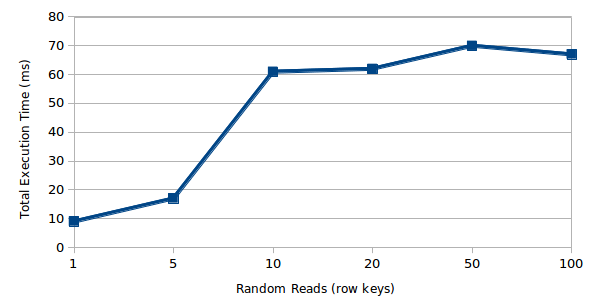
\includegraphics[width=1\textwidth]{./images/randomReads2.png}
\caption{Random row keys reads.} \label{fig:randomReads}
\end{figure}




\bigskip

Figure 6.1 reproduces the obtained results. Although they are not too bad, we can do some more improvements:
\begin{itemize}
\item Configuring block cache:
\par 
HBase has a built-in cache to improve read performance. It just leaves data blocks read from HFiles in a cache if there is enough room for it. It helps reducing disk IO.
\par
 This cache is configurable at columnFamily level, which means that user can choose which columnFamily can be settled in the block cache and which ones not, even user can choose between different cache priorities: \textit{In-Memory}, to try to keep the block in memory more aggressively, \textit{blockCache} = True, the block will be placed within the cache if there is room remaining, and \textit{blockCache} = False, blocks from that columnFamily will not be cached.
\par 
To leverage this feature, we change how our HBase table is created: 
\begin{itemize}
\item For the columnFamily \textit{CF1}, which is the one we want to fetch data, we include \textit{blockCache} = true, and we set it to the highest priority with \textit{In-Memory} = true
\item The rest of the columnFamilies continue as before.
\end{itemize}


\begin{figure}[htb]
\centering
\hspace*{0.21in}
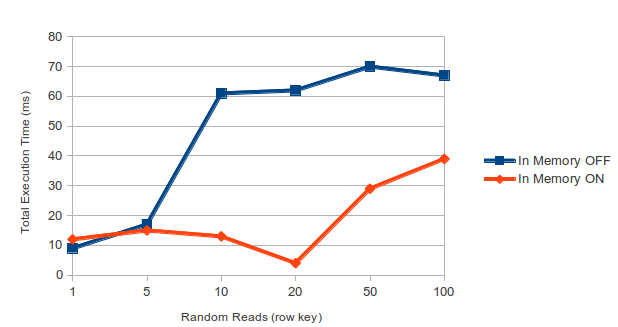
\includegraphics[width=1\textwidth]{./images/inMemory2.png}
\caption{Random row keys Read with and without \textit{In-Memory}.} \label{fig:inMemoryReads}
\end{figure}


Figure 6.2 characterizes \textit{In-Memory} behavior. The total execution time gets reduced if more than 5 rows are retrieved. If we just read once and our requested data is not within the same block, it will be difficult to see how block cache helps, but in a scenario were we would be continuously retrieving 25/50 or more row keys per time this feature would be helpful as there will be data within caches and they will not be empty. 


\item Tuning HFile's block size:
\par
HFile are the actual HBase storage files. Each one is composed of blocks which are the smallest unit of data HBase reads and places in the block cache. These blocks store key/value pairs and have a minimum size, which is by default 64KB. To achieve better performance, we can modified its minimum block size. If we want to improve random reads, we should decrease this value to avoid too many key/value pairs within each block, because the read operation always loads entire blocks and subsequently it looks inside the block for the key/value. Setting it to a lower value will decrease the amount of data fetched by each seek operation, thus decreasing IO and time needed for decompression. On the other hand, it will require more memory to hold the block index, now bigger due to the raise in the number of blocks.

\bigskip

To get the best block size, we have computed the average key/value size of our desired columnFamily (\textit{CF1}).
\par
According to our studies, the average key/value size of the columnFamily \textit{CF1} is hfile.AVG\_KEY\_LEN = 158 bytes + hfile.AVG\_VALUE\_LEN = 52 bytes. For this case the average Key/Value is \textbf{210 bytes}.
\par
64KB turned out to be good enough when dealing with our predefined random reads. Testing it with bigger values (128KB, 256KB) was increasing the latency as expected. In contrast, testing with smaller blocks (32KB, 16KB or 8KB) gave out same or even worse results as with the 64KB value due to HBase is ultimately bound by disk read latency causing bottlenecks when fetching data from disks.

%we had already achieved the level of being bounded by slow disk read latency causing bottlenecks when doing single disk I/O to fetch %data.

\item Bloom Filters:

HBase supports Bloom Filter \cite{bloom1970space}. Bloom Filters are a space-efficient and constant-time mechanism to figure out whether an HFile/storeFile stores a specific row, rowCol cell or not without loading the entire file and scanning the block. They avoid the process of going through each storeFile's block index, which has the start row key of each block inside it, to check whether the row can be there or not, and if it does, then HBase needs to load the block and start scanning it in order to confirm if the row is there or not. The drawback of using Bloom Filter is that it needs to be stored within the HFile and consequently, HFile's size will be boosted. 
\par
By default Bloom Filter is disabled. User just needs to alter the table or create a new one adding the BLOOMFILTER =\textgreater 'ROW' or 'ROWCOL' parameter to enable it. Bloom Filters are configurable at columnFamily level and within it, Bloom Filters can be at row or at row + column level. We set up it at ROW level for the columnFamily CF1 because we are not looking for specific cells, just rows.

\bigskip

Our results do not show and immediate performance gain on our random Get operations since our MapReduce Bulk Load job creates the only necessary and final storeFiles; one storeFile per column family and per Region. In our scenario, we have everything as after a major compaction and HBase does not need to go through each storeFile to get a row since there is only one storeFile to go through. In other scenarios, where there would be a bigger number of storeFiles due to the daily and normal insertions, Bloom Filter mechanism would help skipping the load of lots of storeFiles which would not have the desired row.
\par
Nevertheless, Bloom filters reduce the number of unnecessary block loads, which translate into an improvement in the overall throughput of the entire cluster and that is the reason why we use them.

\end{itemize}

%SUBIR EL ARCHIVO PUT CON -DFG.BLOCKSIZE = 128...256 y listo calisto.


%hbase.mapreduce.hfileoutputformat.blocksize
%The mapreduce HFileOutputFormat writes storefiles/hfiles. This is the minimum hfile blocksize to emit. Usually in hbase, writing hfiles, the blocksize is gotten from the table schema (HColumnDescriptor) but in the mapreduce outputformat context, we don't have access to the schema so get blocksize from Configuration. The smaller you make the blocksize, the bigger your index and the less you fetch on a random-access. Set the blocksize down if you have small cells and want faster random-access of individual cells.








%Meter lo de usar row keys menores etc...longint...en vez de string etc.
%----------------------
%Using bloom filter is almost mandatory there;
%You might also want to try Short Circuit Reads and be sure you get 100\%
%data locality (major compact your table first)
%-------------------
%describir mejor el dataset que tengo..que hay mil de videos repetidos como se puede ver al mirar reduce input groups compare to map output records.
%-----
%lo de los tres ttl (timestamp solo tres)

%\fixme{la tabla de medeiros para test environment, violin-memory (http://www.violin-memory.com/wp-content/uploads/hadoop-benchmark.pdf?d=1)para sacar info de ycsb y read con filter de solo familia. Slurm que caracteristicas pido para mi cluster...}